\documentclass[a4paper]{IEEEtran}

\usepackage{xcolor}
\usepackage{hyperref}
\usepackage[utf8]{inputenc}
\usepackage[pdftex]{graphicx} 

\newcommand\TODO[1]{\textcolor{red}{TODO:#1}}
\newcommand\todo[1]{\TODO{#1}}
\newcommand\cn{\textcolor{red}{[citation needed]}}

\title{The overpowered prefetcher of goodness and excellence!}

\author{
    Sigve Sebastian Farstad,
    Rune Holmgren,
    Torbjørn Langland,
    Per Thomas Lundal
}

\begin{document}

\maketitle

\begin{abstract}
    Le abstract.\cn
\end{abstract}

\section{Introduction}

\todo{ Write briefly about the project, the course it belongs to and the goal}
This is the introduction section.
Here we write something appealing for you to continue on.
If you finish this, you will be baked a cake.

As part of the course TDT4260 Computer Architecture, students in groups of 3 or 4 were to implement and test a prefetcher.
This report describes the implementation with test results done by group 11.
The report will describe the framework for the project, different prefetchers that have been implemented, how they work and the test results.

\section{Related Work}

\todo{ Not sure, mention related work?}
Here we mention related work. Do you want cake for your relatives?

\subsection{Correlation Prefetching}
\todo{write something!}

\subsection{Global History Buffer}
History based prefetchers need to store access patterns efficient data structure that enables quick access.
One such data structure is the Global History Buffer (GHB).
GHB is an $n$-entry First-In, First-Out (FIFO) queue implemented as a circular buffer.
It stores the $n$ most recent L1 cache misses in entries that contain the miss address and a link pointer.
The link pointer is used to chain entries together into time-ordered linked lists that holds the significant access patterns.
An Index Table (IT) is used to keep track of these lists.
It maps some key to the most recent element of a linked list.
The IT is based on a FIFO queue like GHB, but significantly smaller as each entry has to be evaluated for each cache miss to look up a matching key.
The key can be based on any cache miss information, and depending on it a wide variety of history based prefetch methods can be implemented.
In a comparison of different prefetch mechanisms by Péres et al., one using GHB gave the best performance.
\todo{cite MicroLib: a case for the quantitative comparison of micro-architecture mechanisms}
\todo{figure}

\section{Prefetcher Description}
A total of 5 different prefetchers have been implemented and tested. 

\subsection{Delta correlation prediction table}


\subsection{Adaptive program counter delta correlation}

\subsection{Program counter c-zones delta correlation}

\subsection{C-zones delta correlation}

\subsection{Adaptive c-zones delta correlation}

\todo{Describe how the final prefetcher works. I suggest adding a figure. Maybe briefly mention other attempts while if we have space?}

It is common for programs to access datastructures in neatly organized patterns.
In figure \ref{fig:DCExample} values are read with delta values 1 and 9, and this pattern repeats.
Such pattern may be exploited by prefetchers to predict what data will be read next.
A delta correlation prediction table will identify these patterns by comparing the delta values observed on misses with the history for resent misses.
When such patterns are found, the prefetcher will fetch the predicted cachelines into a circular buffer.


\begin{figure}[h!]
  \centering
      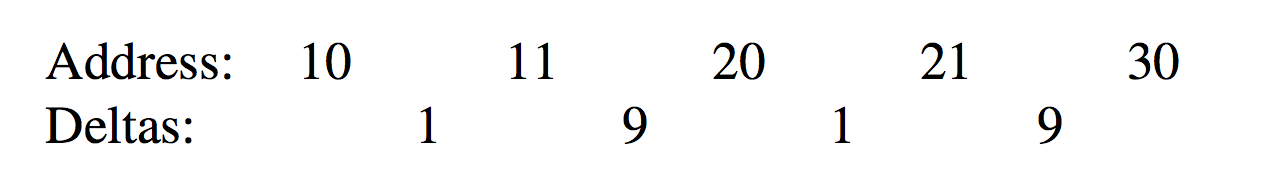
\includegraphics[width=0.5\textwidth]{Figures/DCExample}
  \caption{Delta Correlation Example}
  \label{fig:DCExample}
\end{figure}

As can be seen, the a row in the table contains fields for the PC, last address, last prefetch, deltas 1 to n, and delta pointer.
PC stores the address to the load instruction, and works as index in the table.
The Last Address stores the missed address when there is a miss in the cache.
The delta fields stores the address difference, or the deltas, for each time this instruction is called.
Last prefetch contains the address of the last issued prefetch.
The Delta Pointer points to the head (first Delta field) in the row, since the delta fields are used as circular buffer.

\begin{figure}[h!]
  \centering
      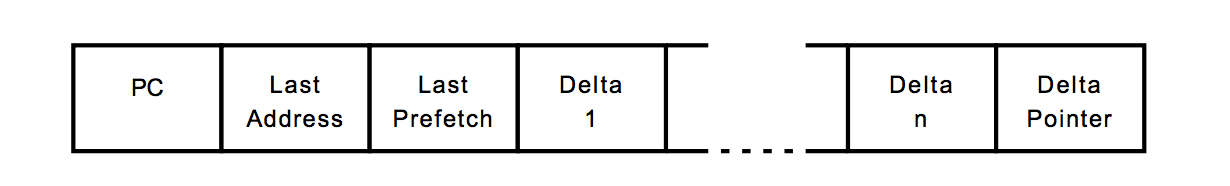
\includegraphics[width=0.5\textwidth]{Figures/DCTable}
  \caption{Delta Correlation Prediction Table}
  \label{fig:DCTable}
\end{figure}

\subsection{Adaptive program counter delta corelation}

\subsection{Program counter c-zones delta corelation}

\subsection{Adaptive c-zones delta corelation}

\subsection{C-zones delta corelation}


\todo{Describe how the final prefetcher works. I suggest adding a figure. Maybe briefly mention other attempts while if we have space?}



Here we describe the cake...uh, I mean the pretecher. Hey, Vance! Can you prefetch that cake?

\section{Methodology}

\todo{Mention the framework. Explain PFJudge. Maybe or maybe not mention C++?}
Here we describe how we did it.

WARNING: Recipee too long. Insert cake recipe here!

\section{Results}

\todo{ Describe results from both local and PFJudge.}

EXPLOSION!

\section{Discussion}

\todo{ Not exactly sure, just say it works better? Compare with other prefetcher IF we chose to describe them. }

You killed GLaDOS.
You monster.

\section{Conclusion}

\todo{ Mention what could have been done better or different? Future ideas? }

The cake is a lie!

\section{Acknowledgements (optional)}

GLaDOS

yoyo \cite{assignment-text}

\bibliography{bibliography}
\bibliographystyle{plain}
\nocite{*}

\end{document}
